\documentclass[../main.tex]{subfiles}

\begin{document}

\section{Filesystem}
\label{section:lauxus:filesystem}

\subsection{Nodes hierarchy}
\label{section:lauxus:filesystem_nodes}

\begin{figure}[ht]
    \centering
    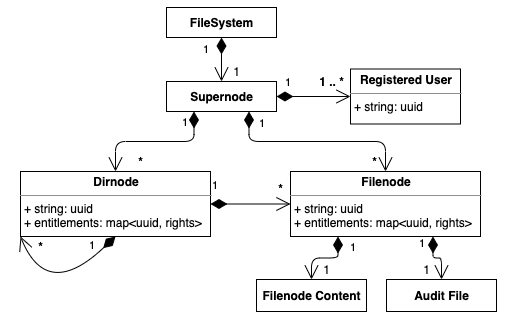
\includegraphics[width=.75\textwidth]{../../images/lauxus/node_hierarchy}
    
    \caption{Nodes UML hierarchy}
    \label{figure:lauxus:nodes_hierarchy}
\end{figure}
\par Our filesystem is composed of different nodes, each one of them representing a standard filesystem entry: either a directory or a file. Every nodes are stored and identified by using a random UUID so that, a curious attacker can't deduce any information about the node's name (e.g: directories named with patients names in the case of our scenario). Thus, our filesystem hierarchy, presented in the following Figure \ref{figure:lauxus:nodes_hierarchy}, is composed of:
\begin{itemize}
    \item A single \textbf{supernode} acting as a user database. It stores a list of all the registered users. This supernode is mainly used as a first firewall for unauthorised users. A secure handshake is initially made before decrypting and opening the filesystem. This handshake and the user management will be covered in its own Section \ref{section:lauxus:login}. Along with this, the supernode is acting as the root directory of the filesystem. Thus, it stores a list of its children nodes. Its children may either be a dirnode or a filenode.
    \item Multiple \textbf{dirnodes}, each representing a standard directory. Each dirnode contains a list of user entitlements describing the user rights to access this specific directory. Further discussion on this entitlement list may be found in Section \ref{section:lauxus:user_entitlement}. In the same way as the supernode, the dirnode stores a list of its children.
    \item Multiple \textbf{filenodes}, each representing a standard file. As well as for a dirnode, they hold an entitlement list. Alongside this, they contain the content of their associated file. Also, they are linked to their corresponding audit files.
\end{itemize}


\subsection{Securing file's content}
\label{section:lauxus:filesystem_encryption}

\par Each file's content must be encrypted in order to be secured from unauthorised parties. As encryption algorithm we are using AES CTR. We chose a simple encryption algorithm instead of an authenticated one because we are not concerned about the file malleability. Indeed, as CTR mode of encryption doesn't produce an authentication tag, an attacker could easily tamper with the file. However, any modifications made by an attacker to the ciphertext will be easily spotted by a user (producing some weird content in the file). Nonetheless, we must cope with the core weakness of CTR mode of encryption: its nonce non re-usability as can be demonstrated in Appendix \ref{appendix:ctr_nonce_weakness}. To palliate to this issue, we must re-encrypt the file on each update. This re-encryption must each time use a new key/IV pair.
\par Re-encrypting the entire file on each update seems extreme and inefficient. To cope with that, we split the file in multiple block. Each block is encrypted with a different key. This way, we have an efficient random file access. Indeed, when there is a file update, we just need to re-encrypt the edited blocks (e.g: when reading 1 byte of a 2GB file, we just need to decrypt the first block - similar with write operation) instead of the entire file.
\par In order to store these block encryption keys we have built a metadata structure that we will be covered in the Section \ref{section:lauxus:metadata}.


\subsection{Filesystem flow}
\label{section:lauxus:filesystem_flow}

\par Before processing \textit{FUSE} requests, the Filesystem API must first do some prepossessing. This process follow the following steps:
\begin{enumerate}
    \item Find the corresponding file's UUID: When mounted, the user sees the filenames in clear. However, they must be obfuscated before storing them on the remote storage. This means that to retrieve the correct file, we must first find the UUID corresponding to the given clear filename.
    \item Check file existence: Once the UUID is known, we must check if the file still exists on the remote storage (in case it has been deleted by a malicious user).
    \item Check the entitlement: Before processing \textit{FUSE} request, we must first check if the current user can execute the \textit{FUSE} action\footnote{Corresponds to a system call: READ, WRITE, UNLINK, GETATTR, etc} on this specific file.
\end{enumerate}

\end{document}